Liu and Truszczynski, 2015, proposed \tit{partial lexicographic preference
trees}, or \tit{PLP-trees}, a language that allows compact representation
of qualitative preferences over combinatorial domains.
In this work, we focus on a slightly adapted version of PLP-trees,
and introduce \tit{partial lexicographic preference forests},
or \tit{PLP-forests}, to reduce the high variance of PLP-trees.
We study applicability of the two preference formalisms 
via empirical experimentation on
learning various classes of PLP-trees from semi-real-world datasets.


\section{Introduction}
Preferences are everywhere and have been extensively studied
by researchers and scientists in artificial intelligence,
psychology, operations research, and social choice theory.

In the recent decade, the interest on preference learning
and approximation has grown stronger with great evidence
in the literature.
Learning conditional preference networks (CP-nets)\cite{boutilier2004cp}
have received tremendous attention.
CP-nets applies intuitive \tit{ceteris paribus} interpretation
of a dependency network of attributes.
However, reasoning tasks for CP-nets are in general
computationally hard, e.g., dominance testing
can be NP-hard when the dependency graph is acyclic\cite{boutilier2004cp},
and is PSPACE-complete when cyclic\cite{goldsmith2008computational}.

AI researchers have also studied learning problems
on preference models with tree structures,
such as lexicographic strategies,
conditional lexicographic trees,
lexicographic preference trees, and
partial lexicographic preference trees.
The general setting for preference learning is the following.
Given a set $\cE$ of pairwise preferences, called \tit{examples},
we want to learn a predicative preference model $\cM$ such that
$\cM$ agrees with as many examples in $\cE$ as possible.
The learned model $\cM$ is predicative in the sense that
it can decide preference orders between unseen outcomes.

Other than the aforementioned models, 
one could also apply supervised learning models in
machine learning, such as decision trees and random
forests.
This requires translation of the examples in $\cE$ to
labeled instances.
For instance, an example $\alpha \succ \beta$ is transformed
to
\begin{center}
	($\alpha$,$\beta$,1) or ($\beta$,$\alpha$,0).
\end{center}

In this work, we focus on a variant of
partial lexicographic preference trees (PLP-trees).
Specifically, we consider four types of PLP-trees,
i.e., UIUP, UICP-1, CIUP-1, and SCICP.

Decision trees are different from partial preference trees.
Although a decision tree is of great value as a machine
learning tool, its size usually grows as there are
more and more training examples, and it does not
directly answer optimal queries.
PLP-trees considered in this work have size polynomial
in the size of the attribute domains.
Computing the optimal outcome given a PLP-tree
also takes polynomial time in the size of these domains.
Moreover, PLP-trees are arguably more intuitive and 
more cognitively plausible than decision trees.


\section{Trees and Forests}
We adapt the class UI-CP different from the original one \cite{conf/aaai15/LiuT}
in the sense that it contains only trees with a partial path where
every node is labeled by a complete CPT.
We should be able to show that, for the adapted UI-CP PLP-tree, 
the \tsc{ConsLearn} problem is in P.  
This case was left open for general UI-CP PLP-trees.


\section{Preference Learning Library}
Here we describe how we built the datasets\footnotemark to 
support preference learning experiments.
We limited the number of issues to 10, and the size of
their domains to 4 if it is more than 4.
The description of the datasets in this library are shown
in \figref{description}.

\footnotetext{\url{http://www.cs.uky.edu/~liu/preflearnlib.php}}

\smallskip \noindent \textbf{BreastCancerWisconsin \ }
The BreastCancerWisconsin dataset has 270 outcomes over 9 attributes.
To generate equivalent and strict examples for the dataset,
we assume that outcomes labeled by ``benign" are better than
those by ``malignant."
For equivalent examples, we have that outcomes labeled by ``benign" are equivalent
to one another, so are those labeled by ``malignant."

\smallskip \noindent \textbf{CarEvaluation \ }
The CarEvaluation dataset has 1728 outcomes over 6 attributes.
To generate equivalent and strict examples for the dataset,
we assume that outcomes labeled by ``vgood" are better than
those by ``good," which are better than those
by ``acc," which are preferred to those by ``unacc."

\smallskip \noindent \textbf{CreditApproval \ }
The CreditApproval dataset has 520 outcomes over 10 attributes.
To generate equivalent and strict examples for the dataset,
we assume that outcomes labeled by ``+" (positive) are better than
those by ``-" (negative).

\smallskip \noindent \textbf{GermanCredit \ }
The GermanCredit dataset has 914 outcomes over 10 attributes.
To generate equivalent and strict examples for the dataset,
we assume that outcomes labeled by ``1" (good) are better than
those by ``2" (bad).

\smallskip \noindent \textbf{Ionosphere \ }
The Ionosphere dataset has 118 outcomes over 10 attributes.
To generate equivalent and strict examples for the dataset,
we assume that outcomes labeled by ``g" (good) are better than
those by ``b" (bad).

\smallskip \noindent \textbf{MammographicMass \ }
The MammographicMass dataset has 118 outcomes over 10 attributes.
To generate equivalent and strict examples for the dataset,
we assume that outcomes labeled by ``0" (benigh) are better than
those by ``1" (malignant).

\smallskip \noindent \textbf{Mushroom \ }
The Mushroom dataset has 184 outcomes over 10 attributes.
To generate equivalent and strict examples for the dataset,
we assume that outcomes labeled by ``e" (edible) are better than
those by ``p" (poisonous).

\smallskip \noindent \textbf{Nursery \ }
The Nursery dataset has 184 outcomes over 10 attributes.
To generate equivalent and strict examples for the dataset,
we assume that outcomes labeled by ``spec\_prior" are better than
those by ``priority," which are better than those
by ``very\_recom," which are preferred to those by ``recommend,"
which again are better than those by ``not\_recom."

\smallskip \noindent \textbf{SPECTHeart \ }
The SPECTHeart dataset has 115 outcomes over 10 attributes.
To generate equivalent and strict examples for the dataset,
we assume that outcomes labeled by ``0" (positive) are better than
those by ``1" (negative).

\smallskip \noindent \textbf{TicTacToe \ }
The TicTacToe dataset has 958 outcomes over 9 attributes.
To generate equivalent and strict examples for the dataset,
we assume that outcomes labeled by ``positive" are better than
those by ``negative".

\smallskip \noindent \textbf{Vehicle \ }
The Vehicle dataset has 455 outcomes over 10 attributes.
To generate equivalent and strict examples for the dataset,
we assume that outcomes labeled by ``bus" are better than
those by ``opel," which are better than those
by ``saab," which are preferred to those by ``van."

\smallskip \noindent \textbf{Wine \ }
The Wine dataset has 455 outcomes over 10 attributes.
To generate equivalent and strict examples for the dataset,
we assume that outcomes labeled by ``1" are better than
those by ``2," which are better than those
by ``3."


\begin{figure*}
	\centering
	\small
	\begin{tabular}{ |c||c|c|c|c| } 
		\hline
		Dataset          & \#Attributes & \#Outcomes & \#StrExamples & \#EqExamples \\
		\hline \hline
		BreastCancerWisconsin   & 9 & 270 & 9,009 & 27,306 \\ 
		\hline
		CarEvaluation           & 6 & 1728 & 682,721 & 809,407\\ 
		\hline
		CreditApproval          & 10 & 520 & 66,079 & 68,861 \\
		\hline
		GermanCredit            & 10 & 914 & 172,368 & 244,873 \\
		\hline
		Ionosphere              & 10 & 118 & 3,472 & 3,431 \\
		\hline
		MammographicMass        & 5 & 62 & 792 & 1,099 \\
		\hline
		Mushroom                & 10 & 184 & 8,448 & 8,388 \\
		\hline
		Nursery                 & 8 & 1,266 & 548,064 & 252,681 \\
		\hline
		SPECTHeart              & 10 & 115 & 3,196 & 3,359 \\
		\hline
		TicTacToe               & 9 & 958 & 207,832 & 250,571 \\
		\hline
		Vehicle                 & 10 & 455 & 76,713 & 26,572 \\
		\hline
		Wine                    & 10 & 177 & 10,322 & 5,254 \\
		\hline
	\end{tabular}
	\caption{Description of datasets in the library}
	\label{fig:description}
\end{figure*}


\section{Experimentation}
We design and implement exact and approximating systems to evaluate PLP-trees and forests of
PLP-trees.

\subsection{Evaluating PLP-Trees}
To evaluate the feasibility of PLP-trees of various classes,
we implemented an exact learner using Answer-Set Programming,
as well as a greedy learning algorithm.

First, for all datasets we achieve results for UIUP PLP-trees
using exact and greedy learning methods, and for decision trees.
For dataset $D$, we randomly pick $\R_D \subset \strictEx$ with $1 \leq |\R_D| \leq 250$
as the set of \tit{training} examples,
and $\T_D = \strictEx \setminus \R_D$ as the set of \tit{testing} examples.
Then, from $\R_D$, we train a UIUP PLP-tree $T_X$ using Answer-Set Programming 
such that $T_X$ decides the most examples in $\R_D$, and another UIUP PLP-tree $T_\MH$ using
greedy heuristic.
To compare our preference trees with decision trees, we also train a decision tree $T_\DT$
from $\R_D$.
Finally, on $\T_D$ we test the models $T_X$, $T_\MH$ and $T_\DT$ to compute the percentages of 
strict examples in $\T_D$ that are correctly decided by them.
This process is repeated $20$ times for all the datasets, and the average results are reported
as \tit{learning curves} presented in \figref{B1}, \figref{Car1}, \figref{Crd1}, 
\figref{G1}, \figref{I1},
\figref{Mam1}, \figref{Mush1}, \figref{S1}, \figref{T1}, \figref{V1}, and \figref{W1}.

\begin{figure*}[ht]
	\centering

  \begin{subfigure}[b]{0.3\textwidth}
		\centering
		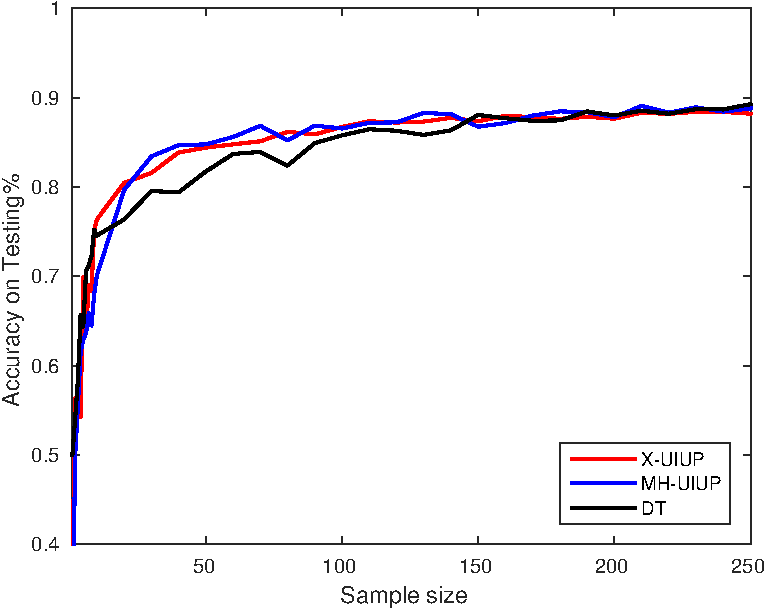
\includegraphics[width=\textwidth]{figs/PLPTF/Trees/BreastCancerWisconsinDownsampled_Trees_X_MH.pdf}
		\caption{BreastCancerWisconsin}
		\label{fig:B1}
	\end{subfigure}
  \begin{subfigure}[b]{0.3\textwidth}
		\centering
  	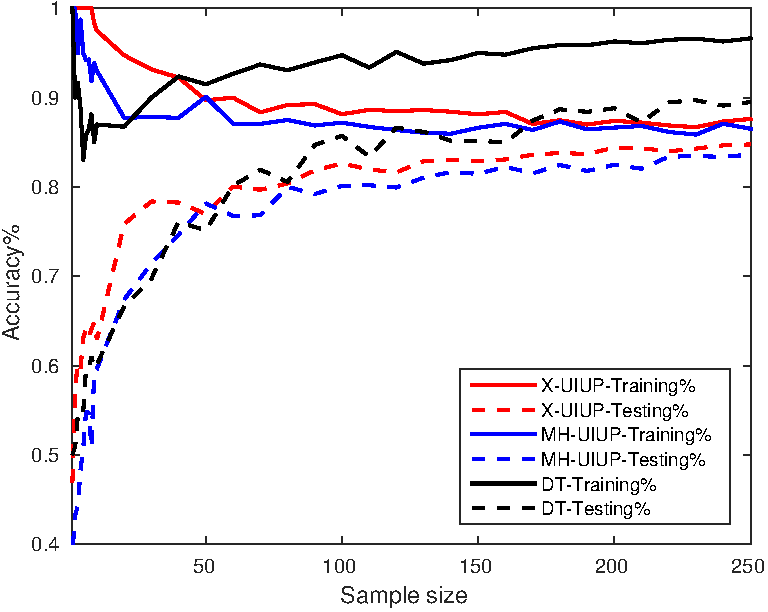
\includegraphics[width=\textwidth]{figs/PLPTF/Trees/CarEvaluation_Trees_X_MH.pdf}
  	\caption{CarEvaluation}
		\label{fig:Car1}
	\end{subfigure}
  \begin{subfigure}[b]{0.3\textwidth}
		\centering
  	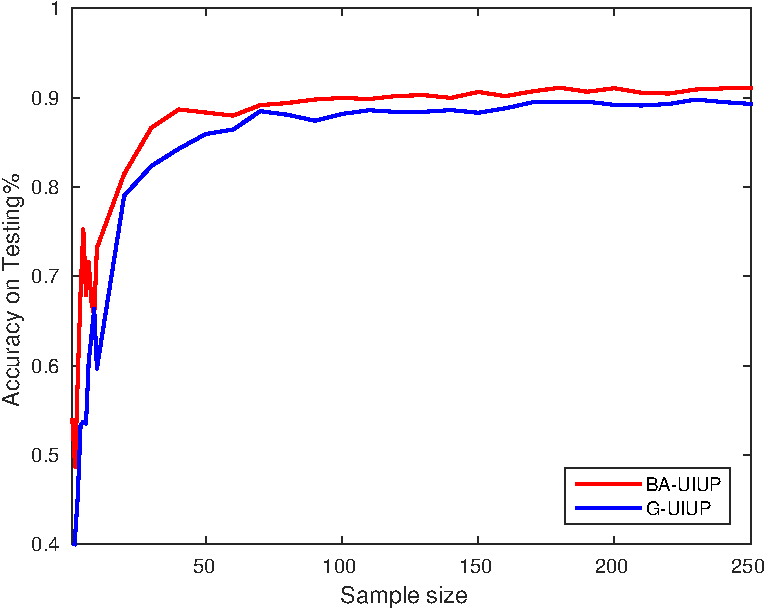
\includegraphics[width=\textwidth]{figs/PLPTF/Trees/CreditApprovalDownsampledFurther_Trees_X_MH.pdf}
  	\caption{CreditApproval}
		\label{fig:Crd1}
	\end{subfigure}
  \\
  \begin{subfigure}[b]{0.3\textwidth}
		\centering
  	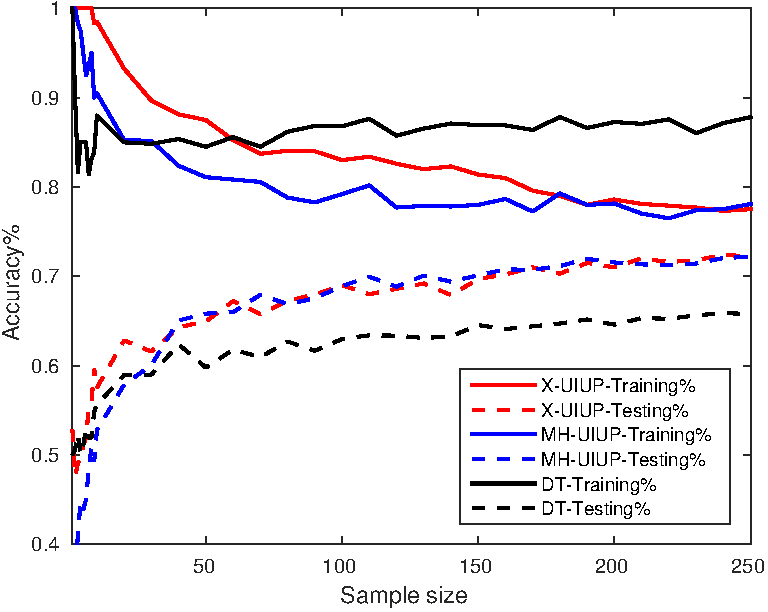
\includegraphics[width=\textwidth]{figs/PLPTF/Trees/GermanCreditDownsampledFurther_Trees_X_MH.pdf}
  	\caption{GermanCredit}
		\label{fig:G1}
	\end{subfigure}
  \begin{subfigure}[b]{0.3\textwidth}
		\centering
  	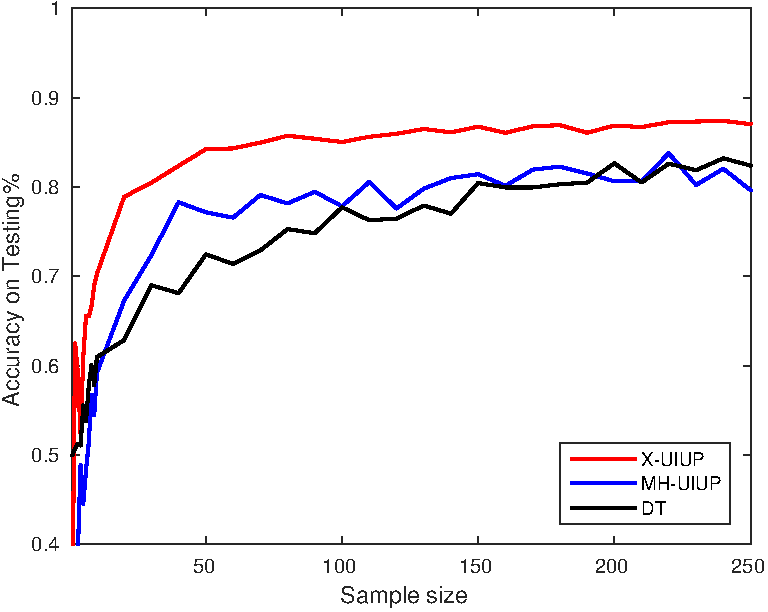
\includegraphics[width=\textwidth]{figs/PLPTF/Trees/IonosphereDownsampledFurther_Trees_X_MH.pdf}
  	\caption{Ionosphere}
		\label{fig:I1}
	\end{subfigure}
  \begin{subfigure}[b]{0.3\textwidth}
		\centering
  	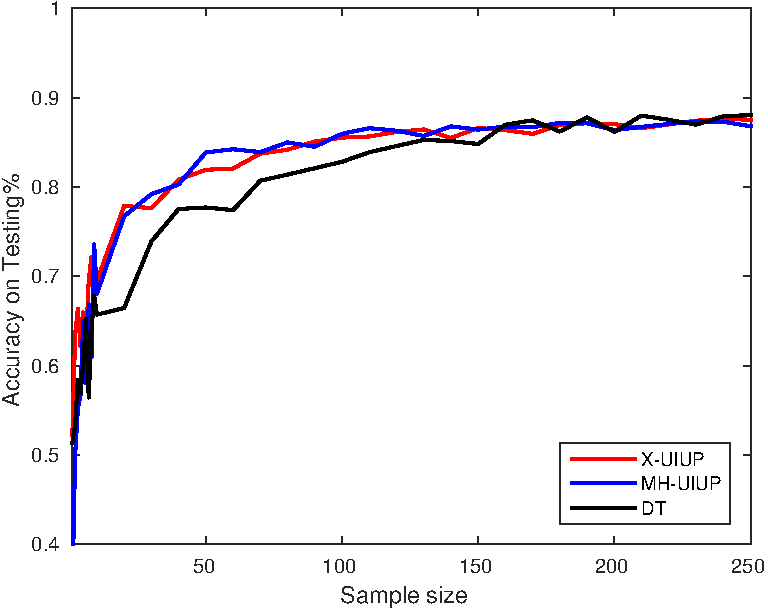
\includegraphics[width=\textwidth]{figs/PLPTF/Trees/MammographicMassDownsampled_Trees_X_MH.pdf}
  	\caption{MammographicMass}
		\label{fig:Mam1}
	\end{subfigure}
	\\
  \begin{subfigure}[b]{0.3\textwidth}
		\centering
  	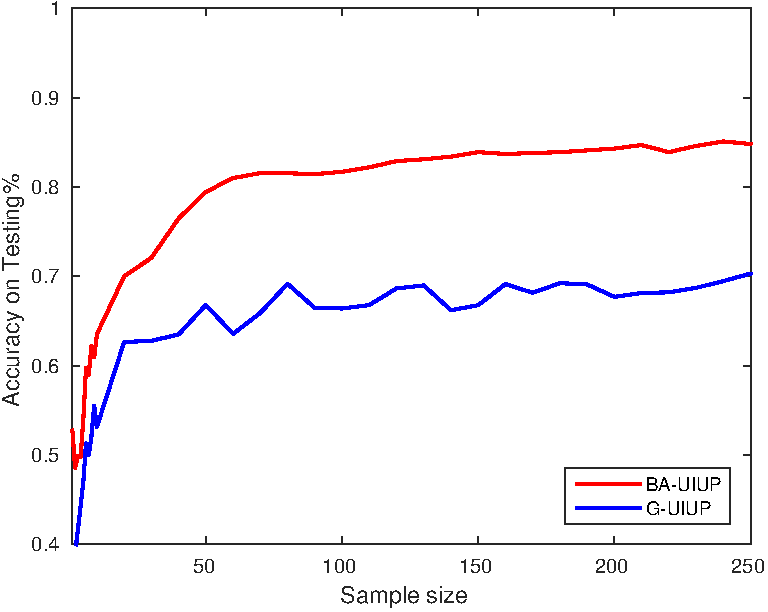
\includegraphics[width=\textwidth]{figs/PLPTF/Trees/MushroomDownsampled_Trees_X_MH.pdf}
  	\caption{Mushroom}
		\label{fig:Mush1}
	\end{subfigure}
  \begin{subfigure}[b]{0.3\textwidth}
		\centering
  	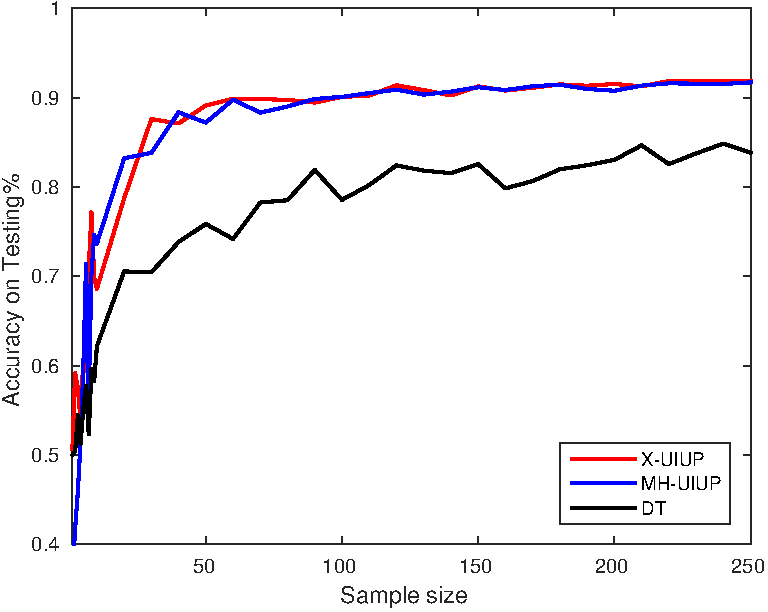
\includegraphics[width=\textwidth]{figs/PLPTF/Trees/NurseryDownsampledFurther_Trees_X_MH.pdf}
  	\caption{Nursery}
		\label{fig:N1}
	\end{subfigure}
  \begin{subfigure}[b]{0.3\textwidth}
		\centering
  	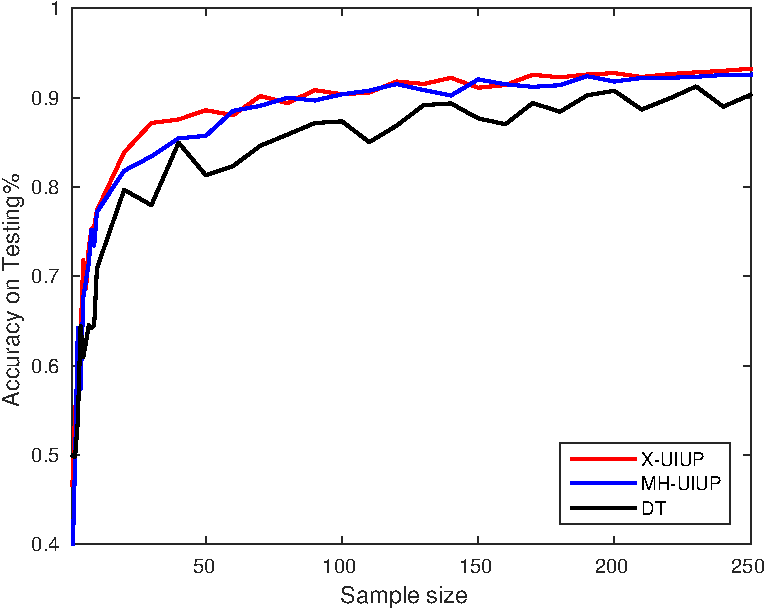
\includegraphics[width=\textwidth]{figs/PLPTF/Trees/SpectHeartDownsampledFurther_Trees_X_MH.pdf}
  	\caption{SpectHeart}
		\label{fig:S1}
	\end{subfigure}
  \\
  \begin{subfigure}[b]{0.3\textwidth}
		\centering
  	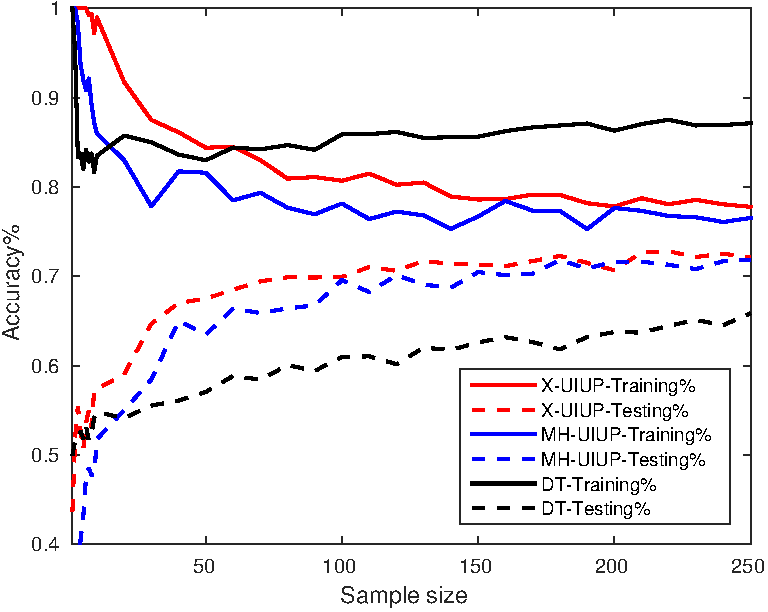
\includegraphics[width=\textwidth]{figs/PLPTF/Trees/TicTacToe_Trees_X_MH.pdf}
  	\caption{TicTacToe}
		\label{fig:T1}
	\end{subfigure}
  \begin{subfigure}[b]{0.3\textwidth}
		\centering
  	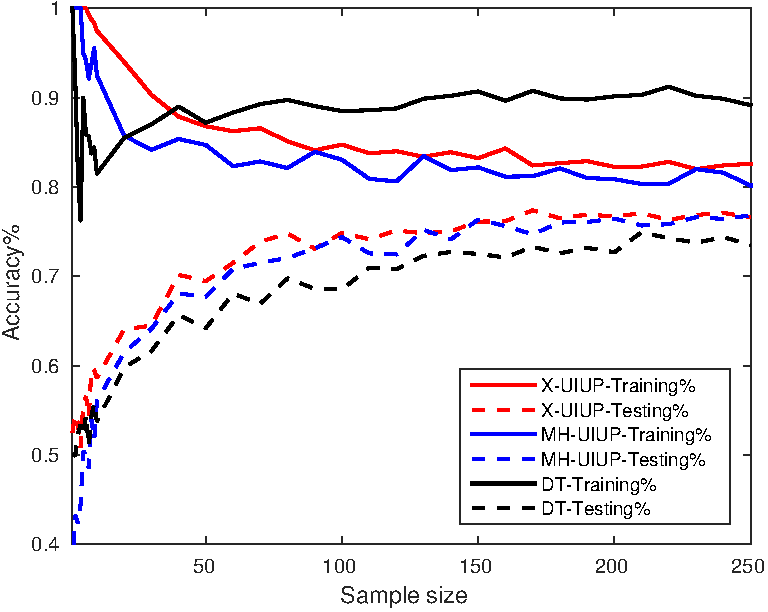
\includegraphics[width=\textwidth]{figs/PLPTF/Trees/VehicleDownsampledFurther_Trees_X_MH.pdf}
  	\caption{Vehicle}
		\label{fig:V1}
	\end{subfigure}
  \begin{subfigure}[b]{0.3\textwidth}
		\centering
  	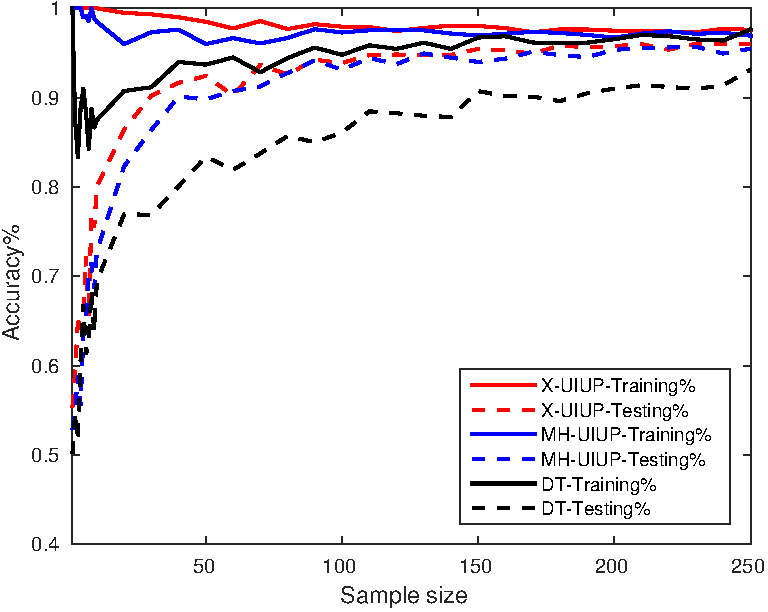
\includegraphics[width=\textwidth]{figs/PLPTF/Trees/WineDownsampled_Trees_X_MH.pdf}
  	\caption{Wine}
		\label{fig:W1}
	\end{subfigure}

  \caption{Learning PLP-trees}
  \label{fig:trees1}
\end{figure*}

Second, we compare the results for UIUP, UICP-1, CIUP-1 and SCICP
PLP-trees using greedy learning.
For dataset $D$, we still generate $R_D$ with $1 \leq |\R_D| \leq 250$ 
and $\T_D$ for training and testing, respectively.
Then, from $\R_D$, we train a UIUP tree $T_1$, $T_2$, $T_3$ and $T_4$ using
the greedy heuristic.
Finally, on $\T_D$ we test the models $T_1$, $T_2$, $T_3$ and $T_4$ to compute the percentages of 
strict examples in $\T_D$ that are correctly decided by them.
This process is repeated 20 times for all the datasets, and the average results are
shown in \figref{B2}, \figref{Car2}, \figref{Crd2}, \figref{G2}, \figref{I2},
\figref{Mam2}, \figref{Mush2}, \figref{S2}, \figref{T2}, \figref{V2}, and \figref{W2}.


\begin{figure*}[ht]
	\centering

  \begin{subfigure}[b]{0.3\textwidth}
		\centering
		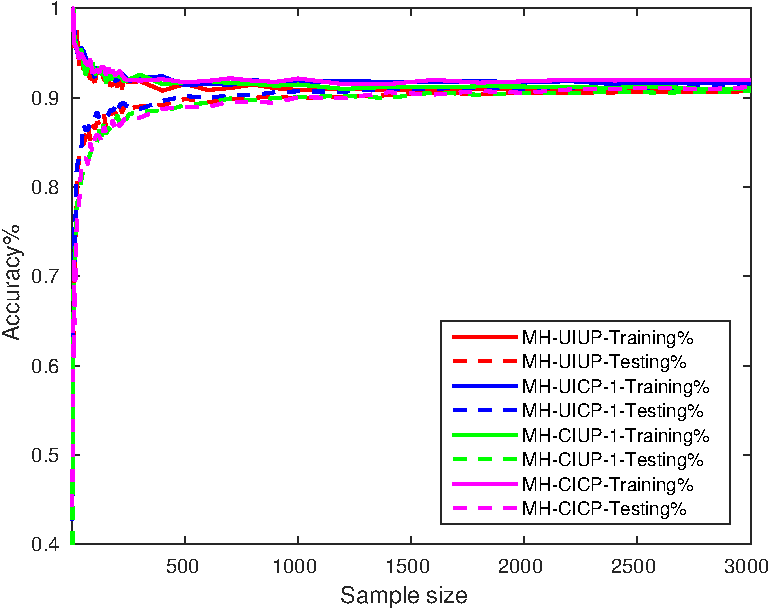
\includegraphics[width=\textwidth]{figs/PLPTF/Trees/BreastCancerWisconsinDownsampled_Trees_MH.pdf}
		\caption{BreastCancerWisconsin}
		\label{fig:B2}
	\end{subfigure}
  \begin{subfigure}[b]{0.3\textwidth}
		\centering
  	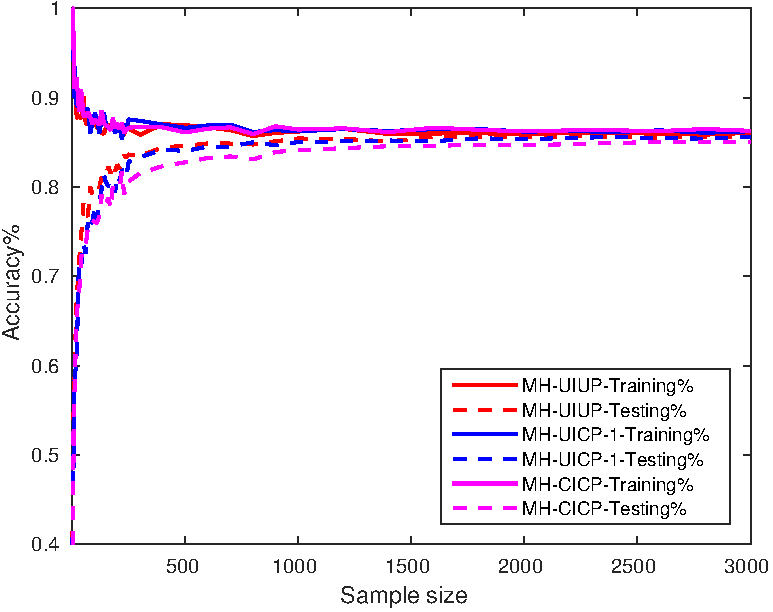
\includegraphics[width=\textwidth]{figs/PLPTF/Trees/CarEvaluation_Trees_MH.pdf}
  	\caption{CarEvaluation}
		\label{fig:Car2}
	\end{subfigure}
  \begin{subfigure}[b]{0.3\textwidth}
		\centering
  	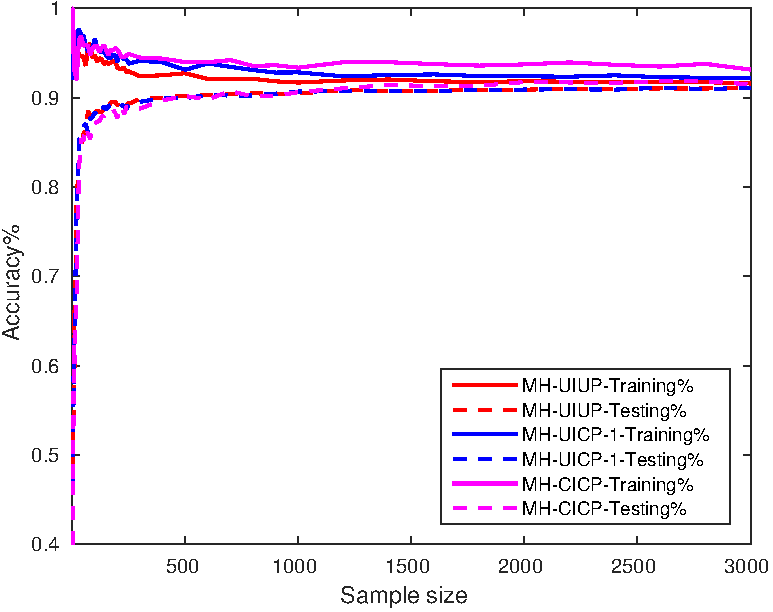
\includegraphics[width=\textwidth]{figs/PLPTF/Trees/CreditApprovalDownsampledFurther_Trees_MH.pdf}
  	\caption{CreditApproval}
		\label{fig:Crd2}
	\end{subfigure}
  \\
  \begin{subfigure}[b]{0.3\textwidth}
		\centering
  	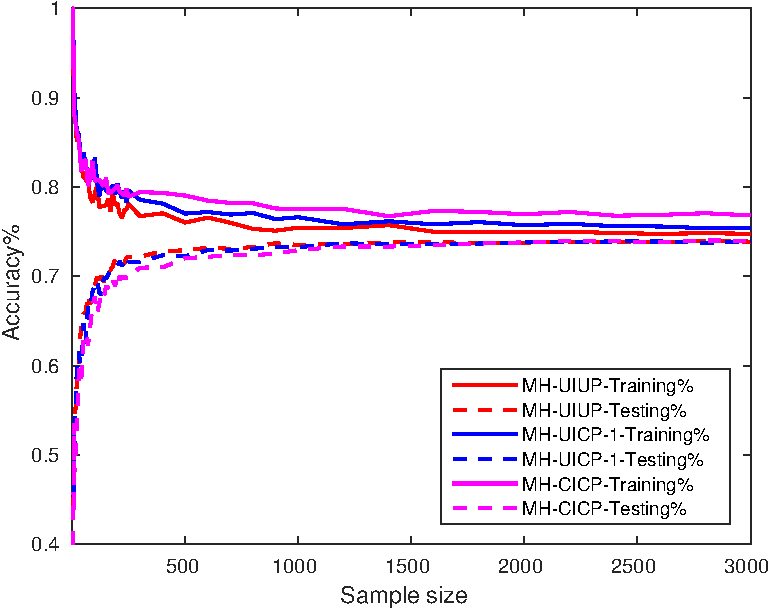
\includegraphics[width=\textwidth]{figs/PLPTF/Trees/GermanCreditDownsampledFurther_Trees_MH.pdf}
  	\caption{GermanCredit}
		\label{fig:G2}
	\end{subfigure}
  \begin{subfigure}[b]{0.3\textwidth}
		\centering
  	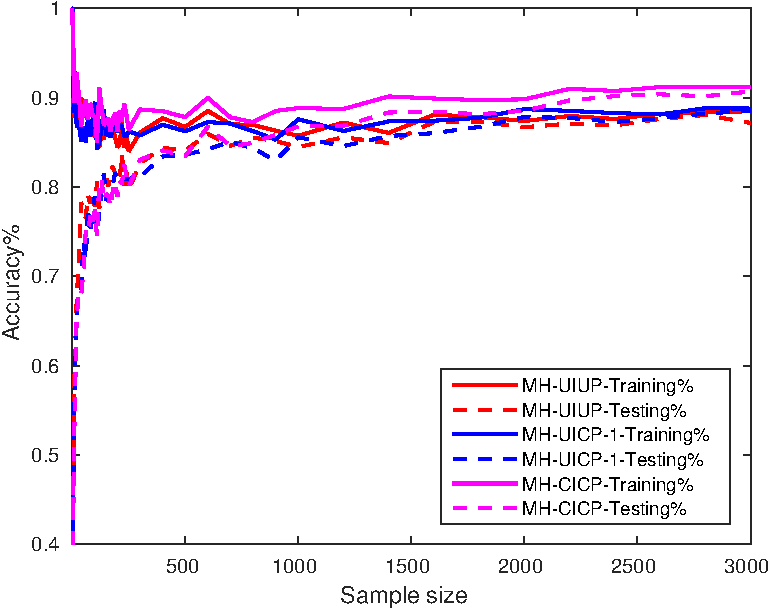
\includegraphics[width=\textwidth]{figs/PLPTF/Trees/IonosphereDownsampledFurther_Trees_MH.pdf}
  	\caption{Ionosphere}
		\label{fig:I2}
	\end{subfigure}
  \begin{subfigure}[b]{0.3\textwidth}
		\centering
  	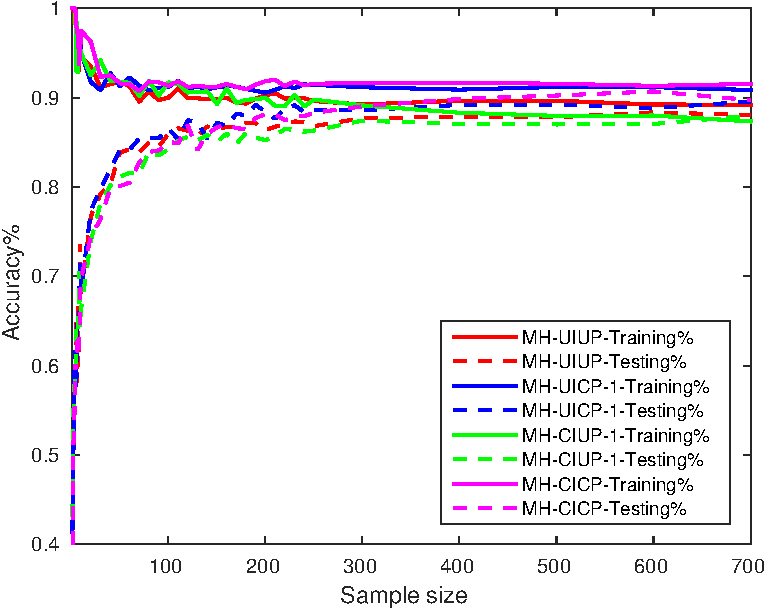
\includegraphics[width=\textwidth]{figs/PLPTF/Trees/MammographicMassDownsampled_Trees_MH.pdf}
  	\caption{MammographicMass}
		\label{fig:Mam2}
	\end{subfigure}
	\\
  \begin{subfigure}[b]{0.3\textwidth}
		\centering
  	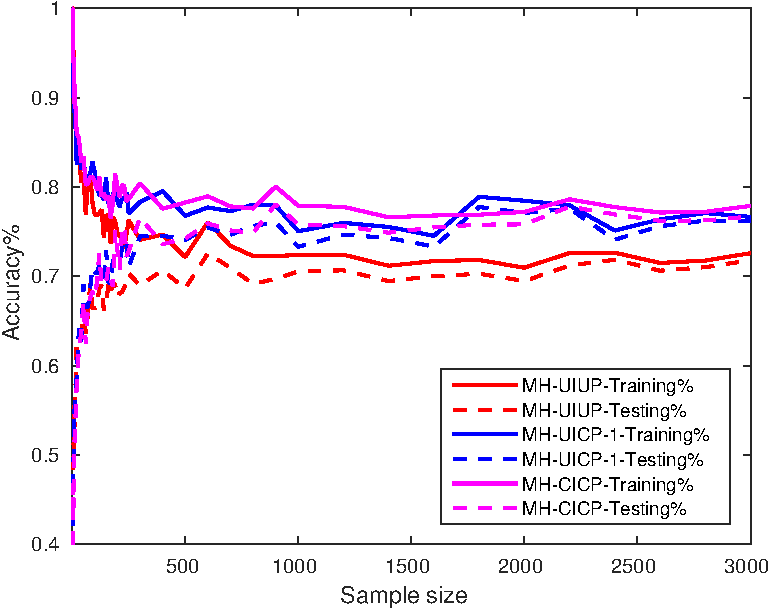
\includegraphics[width=\textwidth]{figs/PLPTF/Trees/MushroomDownsampled_Trees_MH.pdf}
  	\caption{Mushroom}
		\label{fig:Mush2}
	\end{subfigure}
  \begin{subfigure}[b]{0.3\textwidth}
		\centering
  	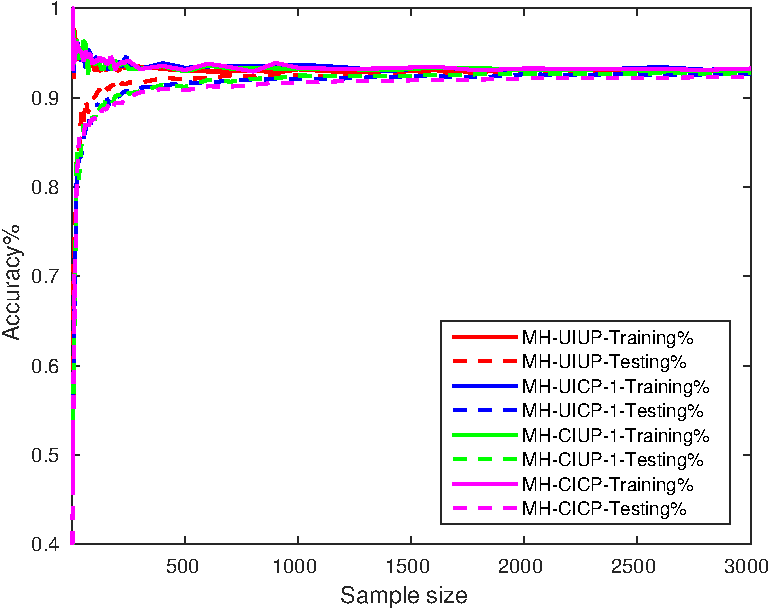
\includegraphics[width=\textwidth]{figs/PLPTF/Trees/NurseryDownsampledFurther_Trees_MH.pdf}
  	\caption{Nursery}
		\label{fig:N2}
	\end{subfigure}
  \begin{subfigure}[b]{0.3\textwidth}
		\centering
  	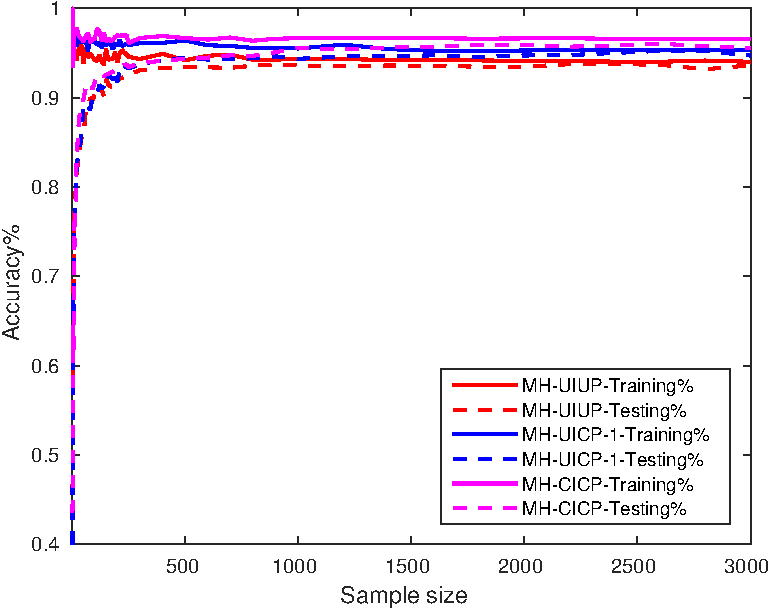
\includegraphics[width=\textwidth]{figs/PLPTF/Trees/SpectHeartDownsampledFurther_Trees_MH.pdf}
  	\caption{SpectHeart}
		\label{fig:S2}
	\end{subfigure}
  \\
  \begin{subfigure}[b]{0.3\textwidth}
		\centering
  	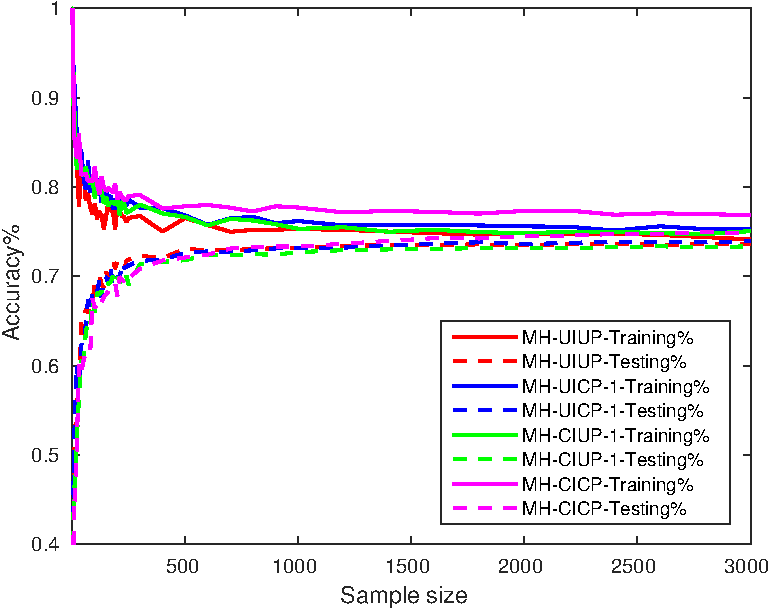
\includegraphics[width=\textwidth]{figs/PLPTF/Trees/TicTacToe_Trees_MH.pdf}
  	\caption{TicTacToe}
		\label{fig:T2}
	\end{subfigure}
  \begin{subfigure}[b]{0.3\textwidth}
		\centering
  	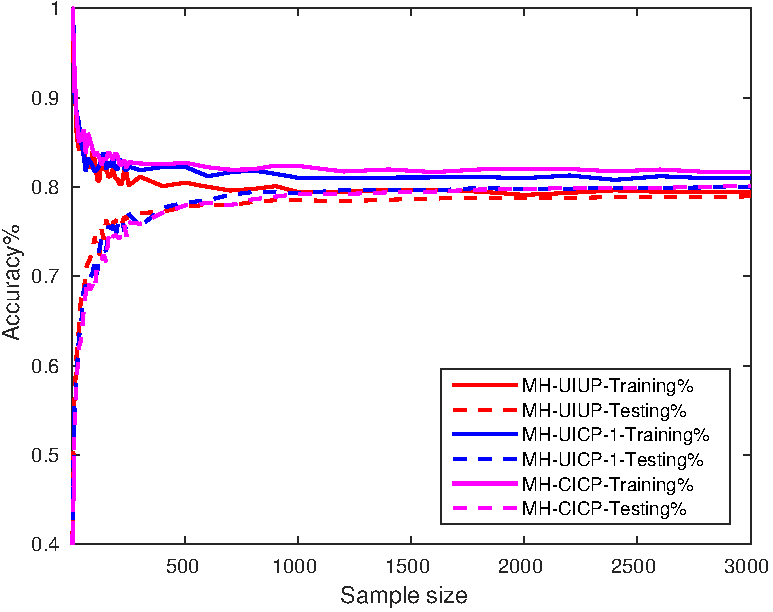
\includegraphics[width=\textwidth]{figs/PLPTF/Trees/VehicleDownsampledFurther_Trees_MH.pdf}
  	\caption{Vehicle}
		\label{fig:V2}
	\end{subfigure}
  \begin{subfigure}[b]{0.3\textwidth}
		\centering
  	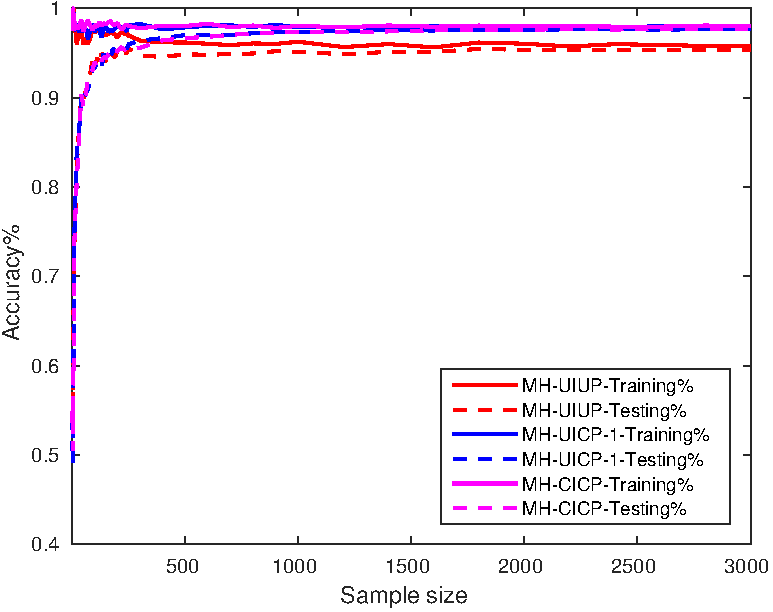
\includegraphics[width=\textwidth]{figs/PLPTF/Trees/WineDownsampled_Trees_MH.pdf}
  	\caption{Wine}
		\label{fig:W2}
	\end{subfigure}

  \caption{Learning Various Types of PLP-trees}
  \label{fig:trees2}
\end{figure*}

\subsection{Evaluating PLP-Forests}
We introduce the notion of \tit{PLP-forests} that is a collection of
PLP-trees.
Let $F$ be a PLP-forest such that $F = \{T_1,\ldots,T_n\}$.
Let us denote by $N_F(o_1,o_2)=|\{T \in F:o_1 \succ_T o_2\}|$.
Now consider the dominance testing problem.
Given a preference forest $F$, and two outcomes $o_1$ and $o_2$,
we say that $o_1 \succ_F^\Maj o_2$ iff $N_F(o_1,o_2)>N_F(o_2,o_1)$,
and that $o_1 \approx_F^\Maj o_2$ iff $N_F(o_1,o_2)=N_F(o_2,o_1)$,
where $\Maj$ stands for the majority rule.
Indeed, the majority rule is an intuitive and computationally easy
preference aggregation rule.
In general, however, it may lead to the so-called Condorcet paradox, where
the $\succ_F^\Maj$ relation contains a cycle.
Other aggregation method could be investigated are positional
scoring rules (adjusted for total \tit{preorders}), Copeland's
method, among others.

First, we show results for UIUP PLP-forests using exact learning
and the greedy heuristic.
In each experiment, we randomly partition a dataset into training
set (70\%) and testing set (30\%), learn a forest (the size of it
indicated by on the x-axis) where
each tree is learned from 50 randomly selected examples from the
training set, and test the forest against the testing set.
We repeat it 20 times and report the averge accuracy (indicated on
the y-axis) in the plots.
Note that the plots also include a straight line representing
the result for learning a UIUP PLP-tree, had we used all the
training data to learn a single tree using the greedy heuristic.
These results are shown in \figref{B3}, \figref{Car3}, \figref{Crd3}, \figref{I3},
\figref{Mam3}, \figref{S3}, \figref{T3}, \figref{V3}, and \figref{W3}.

\begin{figure*}[ht]
	\centering

  \begin{subfigure}[b]{0.3\textwidth}
		\centering
		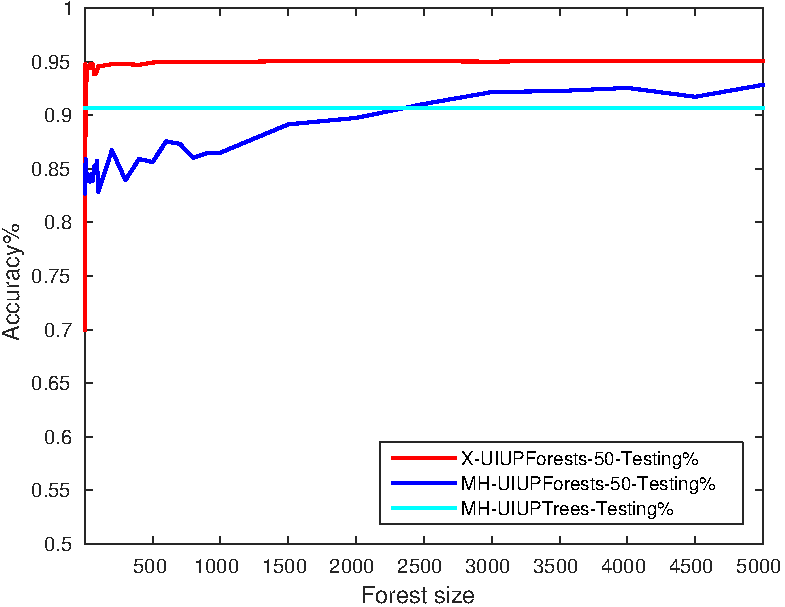
\includegraphics[width=\textwidth]{figs/PLPTF/Forests/BreastCancerWisconsinDownsampled_Forests_X_MH.pdf}
		\caption{BreastCancerWisconsin}
		\label{fig:B3}
	\end{subfigure}
  \begin{subfigure}[b]{0.3\textwidth}
		\centering
  	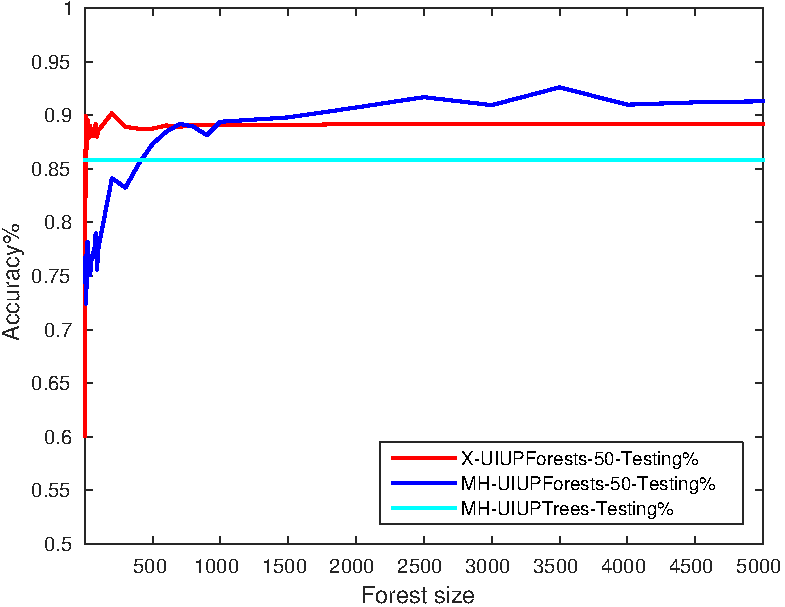
\includegraphics[width=\textwidth]{figs/PLPTF/Forests/CarEvaluation_Forests_X_MH.pdf}
  	\caption{CarEvaluation}
		\label{fig:Car3}
	\end{subfigure}
  \begin{subfigure}[b]{0.3\textwidth}
		\centering
  	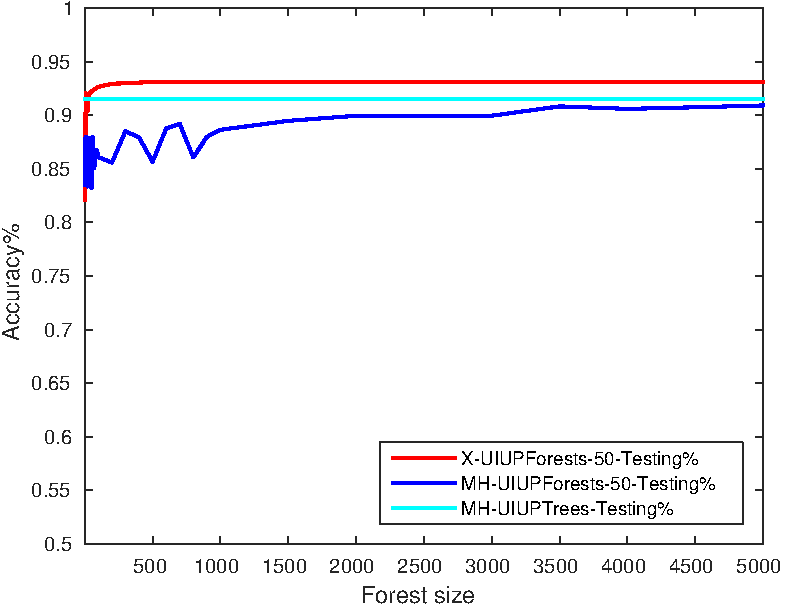
\includegraphics[width=\textwidth]{figs/PLPTF/Forests/CreditApprovalDownsampledFurther_Forests_X_MH.pdf}
  	\caption{CreditApproval}
		\label{fig:Crd3}
	\end{subfigure}
  \\
  \begin{subfigure}[b]{0.3\textwidth}
		\centering
  	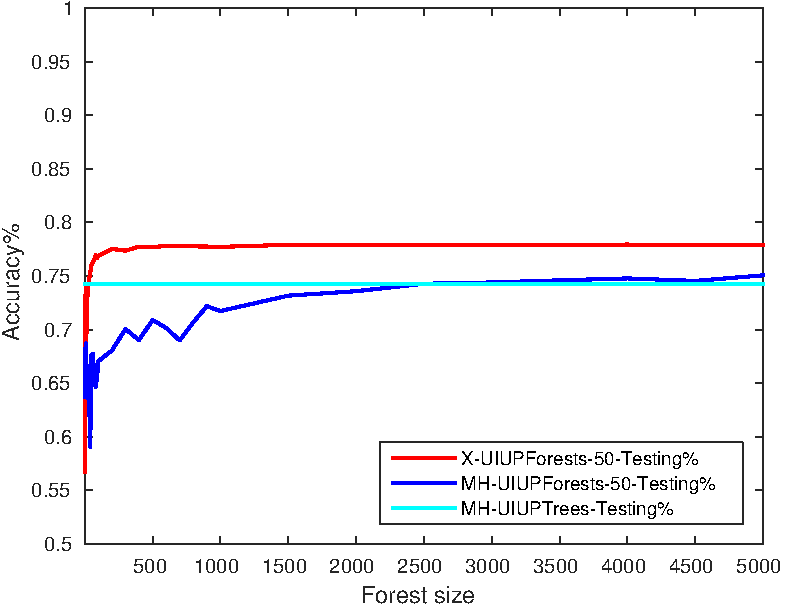
\includegraphics[width=\textwidth]{figs/PLPTF/Forests/GermanCreditDownsampledFurther_Forests_X_MH.pdf}
  	\caption{GermanCredit}
		\label{fig:G3}
	\end{subfigure}
  \begin{subfigure}[b]{0.3\textwidth}
		\centering
  	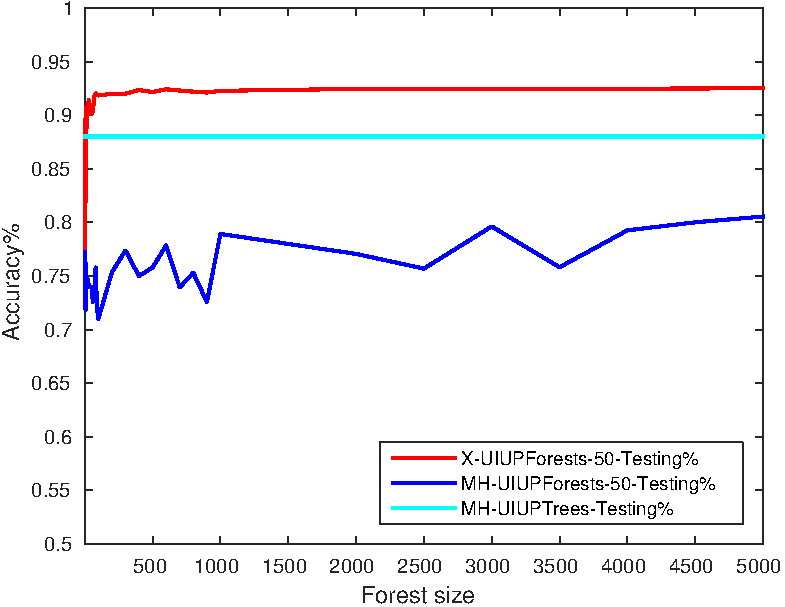
\includegraphics[width=\textwidth]{figs/PLPTF/Forests/IonosphereDownsampledFurther_Forests_X_MH.pdf}
  	\caption{Ionosphere}
		\label{fig:I3}
	\end{subfigure}
  \begin{subfigure}[b]{0.3\textwidth}
		\centering
  	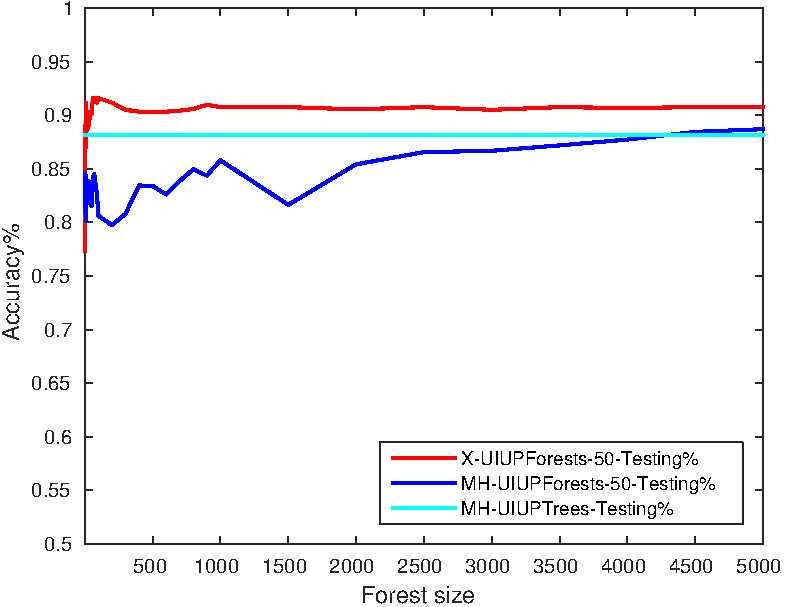
\includegraphics[width=\textwidth]{figs/PLPTF/Forests/MammographicMassDownsampled_Forests_X_MH.pdf}
  	\caption{MammographicMass}
		\label{fig:Mam3}
	\end{subfigure}
	\\
  \begin{subfigure}[b]{0.3\textwidth}
		\centering
  	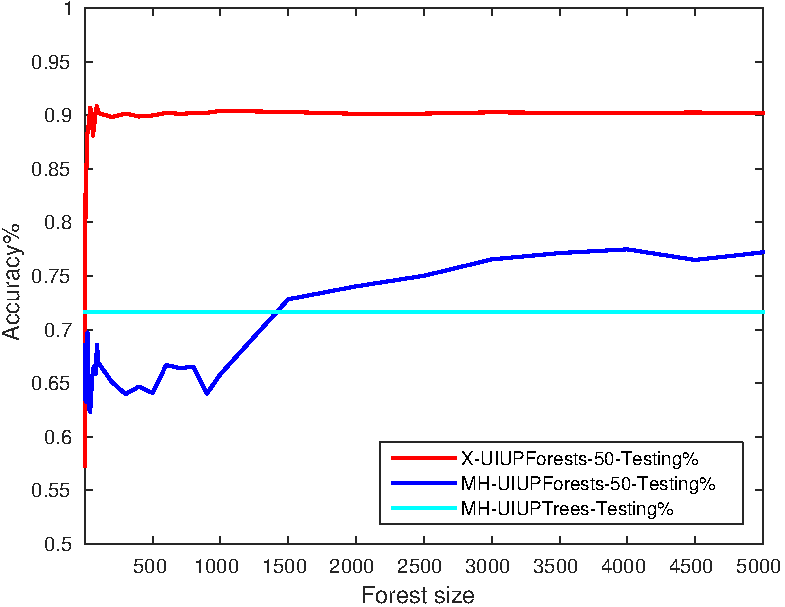
\includegraphics[width=\textwidth]{figs/PLPTF/Forests/MushroomDownsampled_Forests_X_MH.pdf}
  	\caption{Mushroom}
		\label{fig:Mush3}
	\end{subfigure}
  \begin{subfigure}[b]{0.3\textwidth}
		\centering
  	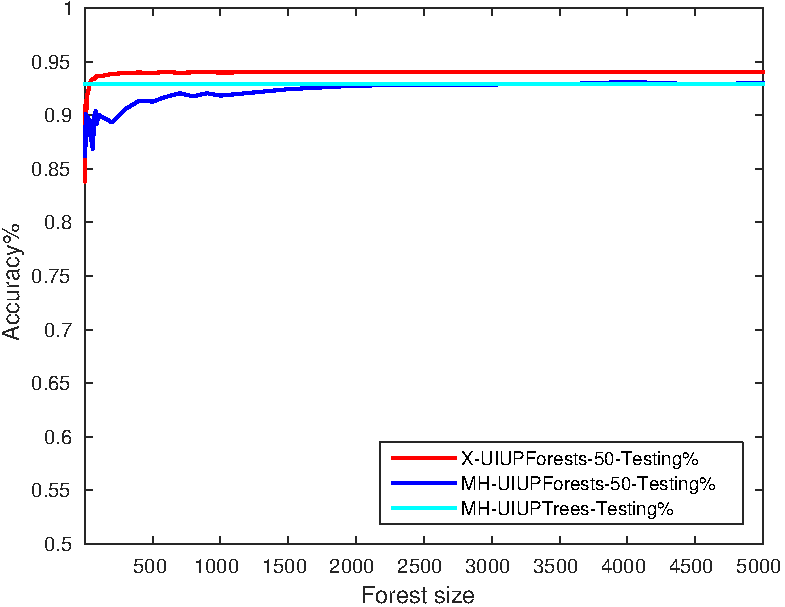
\includegraphics[width=\textwidth]{figs/PLPTF/Forests/NurseryDownsampledFurther_Forests_X_MH.pdf}
  	\caption{Nursery}
		\label{fig:N3}
	\end{subfigure}
  \begin{subfigure}[b]{0.3\textwidth}
		\centering
  	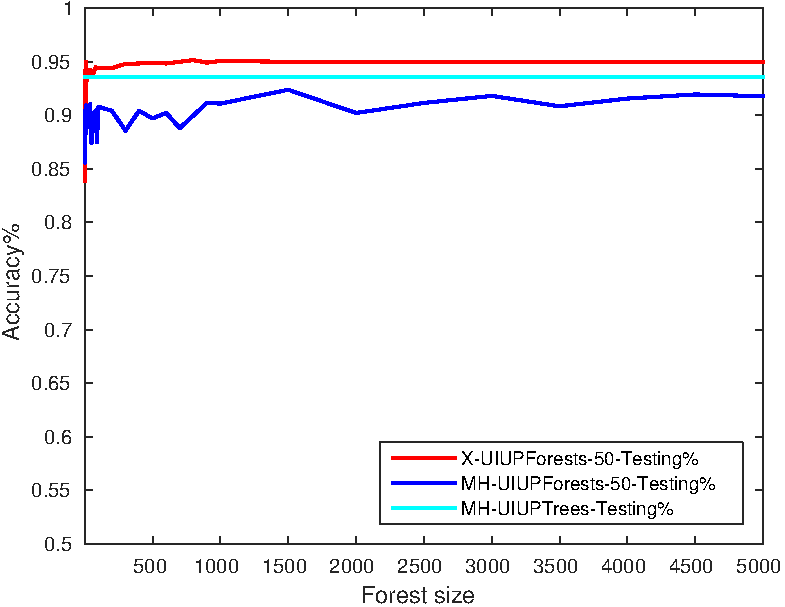
\includegraphics[width=\textwidth]{figs/PLPTF/Forests/SpectHeartDownsampledFurther_Forests_X_MH.pdf}
  	\caption{SpectHeart}
		\label{fig:S3}
	\end{subfigure}
  \\
  \begin{subfigure}[b]{0.3\textwidth}
		\centering
  	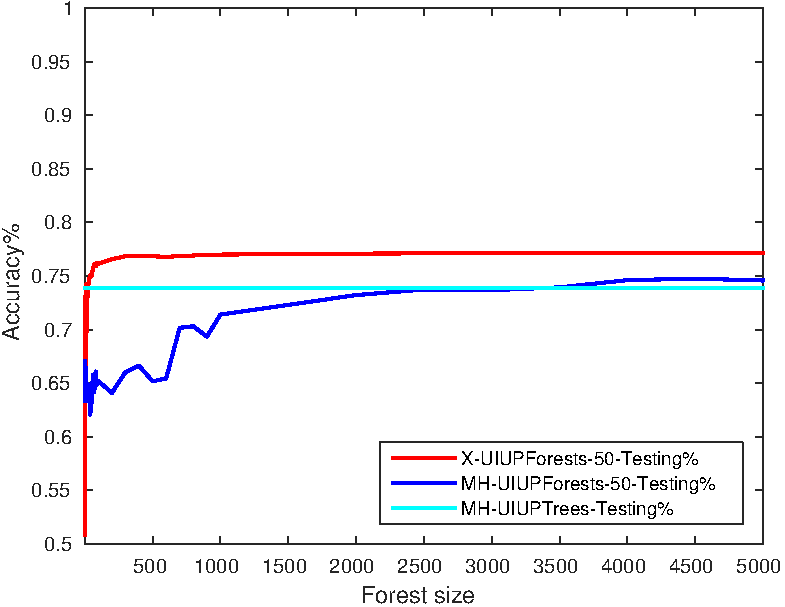
\includegraphics[width=\textwidth]{figs/PLPTF/Forests/TicTacToe_Forests_X_MH.pdf}
  	\caption{TicTacToe}
		\label{fig:T3}
	\end{subfigure}
  \begin{subfigure}[b]{0.3\textwidth}
		\centering
  	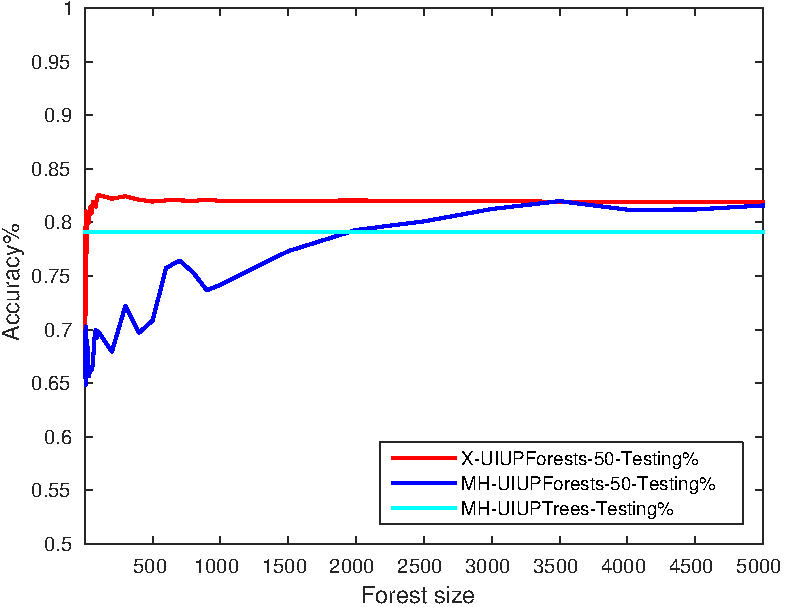
\includegraphics[width=\textwidth]{figs/PLPTF/Forests/VehicleDownsampledFurther_Forests_X_MH.pdf}
  	\caption{Vehicle}
		\label{fig:V3}
	\end{subfigure}
  \begin{subfigure}[b]{0.3\textwidth}
		\centering
  	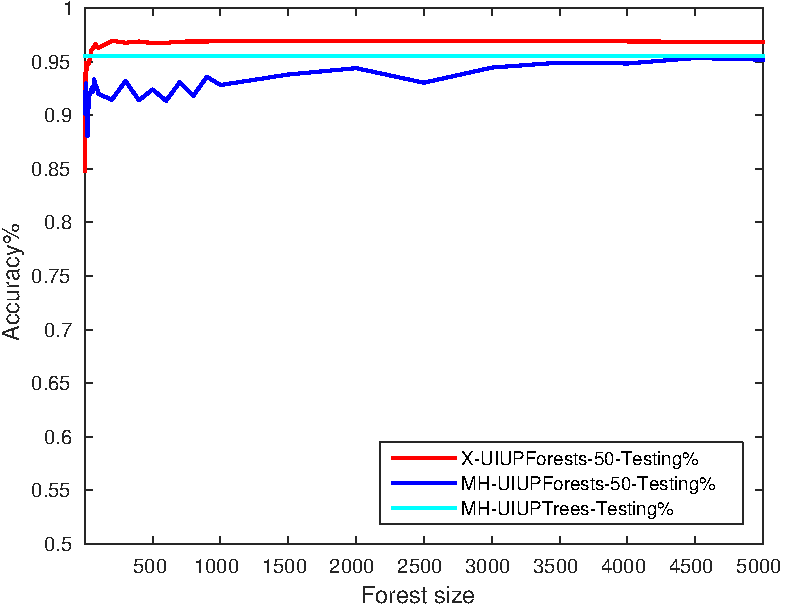
\includegraphics[width=\textwidth]{figs/PLPTF/Forests/WineDownsampled_Forests_X_MH.pdf}
  	\caption{Wine}
		\label{fig:W3}
	\end{subfigure}

  \caption{Learning Forests of PLP-trees}
  \label{fig:forests1}
\end{figure*}

Second, we show results for UIUP PLP-forests using the greedy
heuristic with different learning sample size per tree.
The setting is similar to the previous one.
These results are shown in \figref{B4}, \figref{Car4}, \figref{Crd4}, \figref{I4},
\figref{Mam4}, \figref{S4}, \figref{T4}, \figref{V4}, and \figref{W4}.

\begin{figure*}[ht]
	\centering

  \begin{subfigure}[b]{0.3\textwidth}
		\centering
		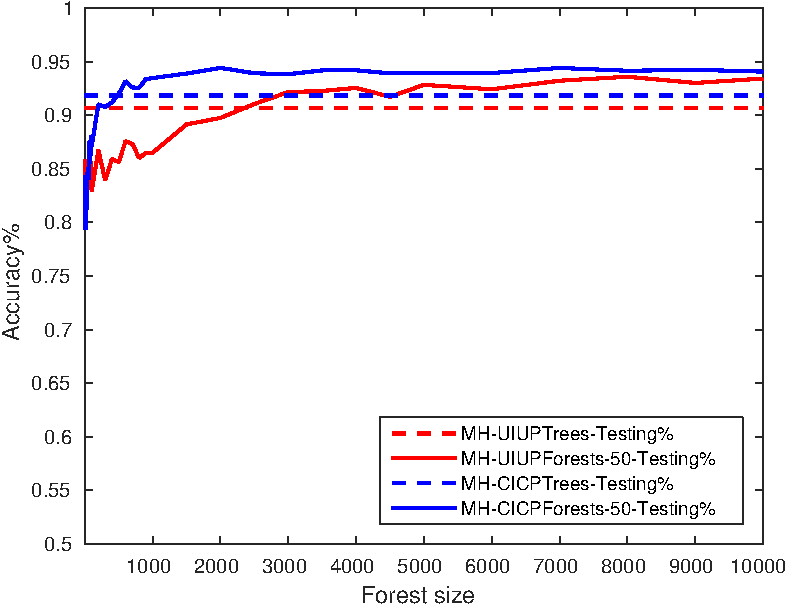
\includegraphics[width=\textwidth]{figs/PLPTF/Forests/BreastCancerWisconsinDownsampled_Forests_MH.pdf}
		\caption{BreastCancerWisconsin}
		\label{fig:B4}
	\end{subfigure}
  \begin{subfigure}[b]{0.3\textwidth}
		\centering
  	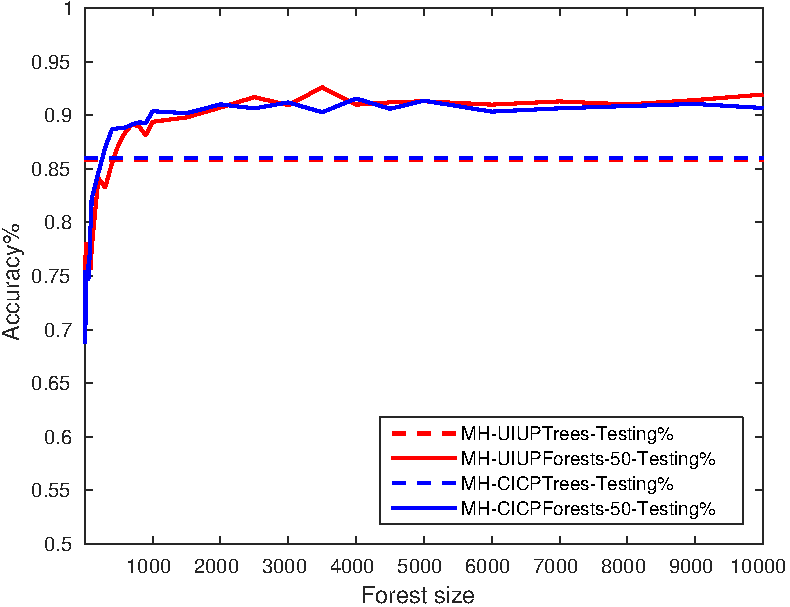
\includegraphics[width=\textwidth]{figs/PLPTF/Forests/CarEvaluation_Forests_MH.pdf}
  	\caption{CarEvaluation}
		\label{fig:Car4}
	\end{subfigure}
  \begin{subfigure}[b]{0.3\textwidth}
		\centering
  	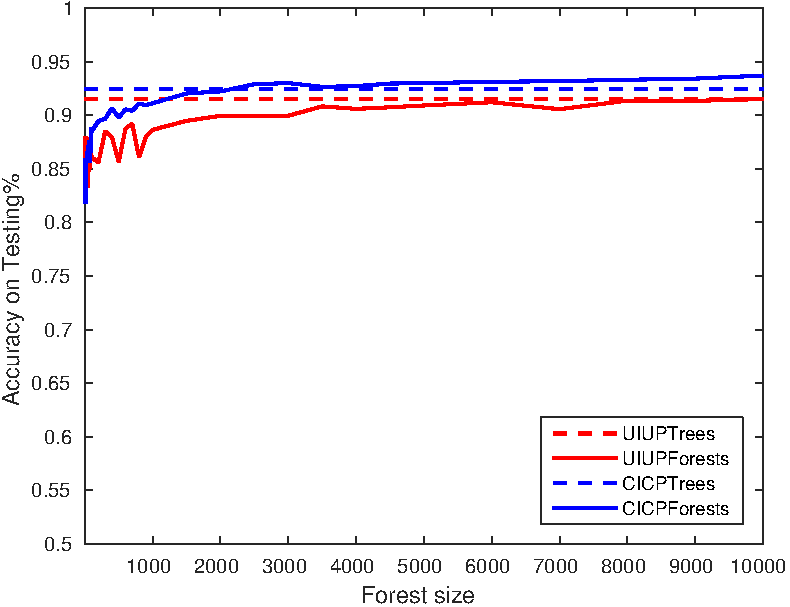
\includegraphics[width=\textwidth]{figs/PLPTF/Forests/CreditApprovalDownsampledFurther_Forests_MH.pdf}
  	\caption{CreditApproval}
		\label{fig:Crd4}
	\end{subfigure}
  \\
  \begin{subfigure}[b]{0.3\textwidth}
		\centering
  	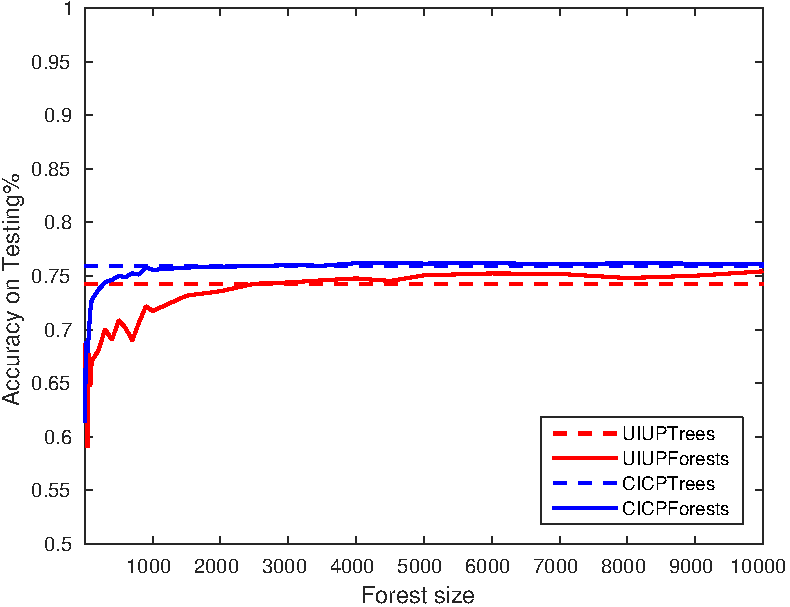
\includegraphics[width=\textwidth]{figs/PLPTF/Forests/GermanCreditDownsampledFurther_Forests_MH.pdf}
  	\caption{GermanCredit}
		\label{fig:G4}
	\end{subfigure}
  \begin{subfigure}[b]{0.3\textwidth}
		\centering
  	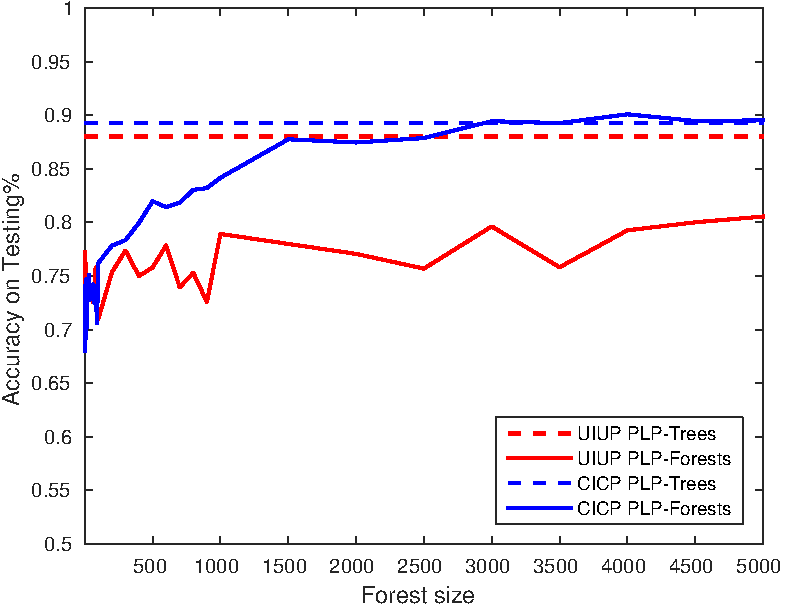
\includegraphics[width=\textwidth]{figs/PLPTF/Forests/IonosphereDownsampledFurther_Forests_MH.pdf}
  	\caption{Ionosphere}
		\label{fig:I4}
	\end{subfigure}
  \begin{subfigure}[b]{0.3\textwidth}
		\centering
  	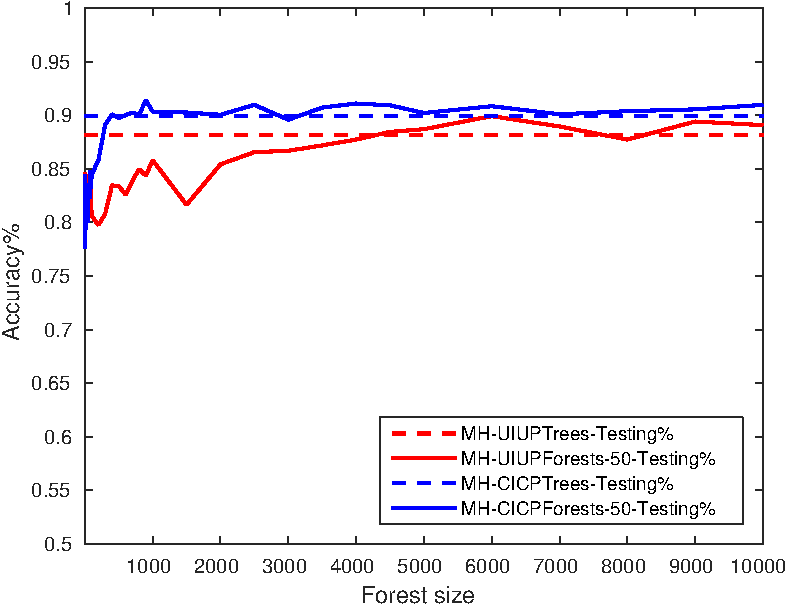
\includegraphics[width=\textwidth]{figs/PLPTF/Forests/MammographicMassDownsampled_Forests_MH.pdf}
  	\caption{MammographicMass}
		\label{fig:Mam4}
	\end{subfigure}
	\\
  \begin{subfigure}[b]{0.3\textwidth}
		\centering
  	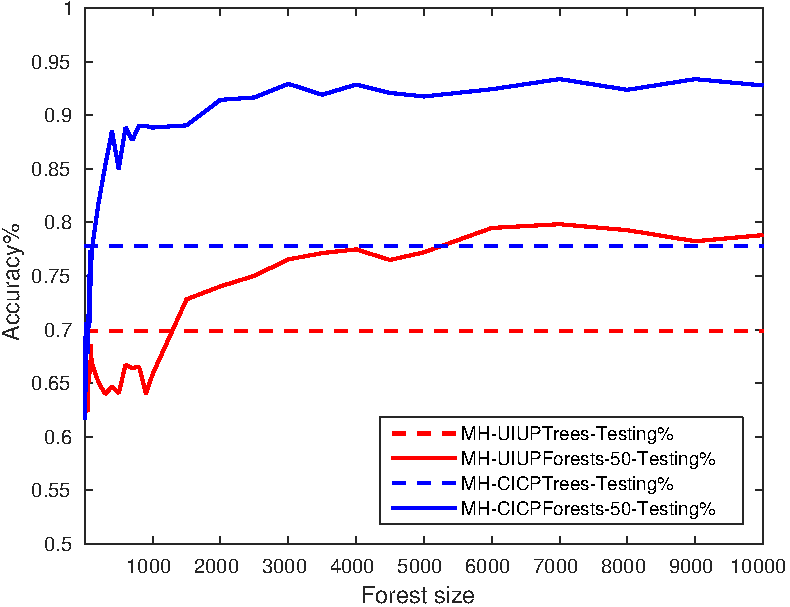
\includegraphics[width=\textwidth]{figs/PLPTF/Forests/MushroomDownsampled_Forests_MH.pdf}
  	\caption{Mushroom}
		\label{fig:Mush4}
	\end{subfigure}
  \begin{subfigure}[b]{0.3\textwidth}
		\centering
  	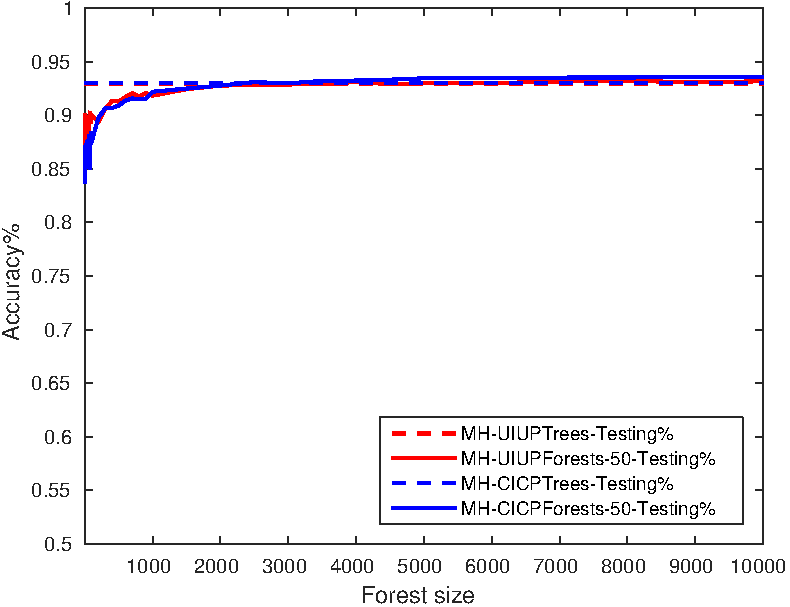
\includegraphics[width=\textwidth]{figs/PLPTF/Forests/NurseryDownsampledFurther_Forests_MH.pdf}
  	\caption{Nursery}
		\label{fig:N4}
	\end{subfigure}
  \begin{subfigure}[b]{0.3\textwidth}
		\centering
  	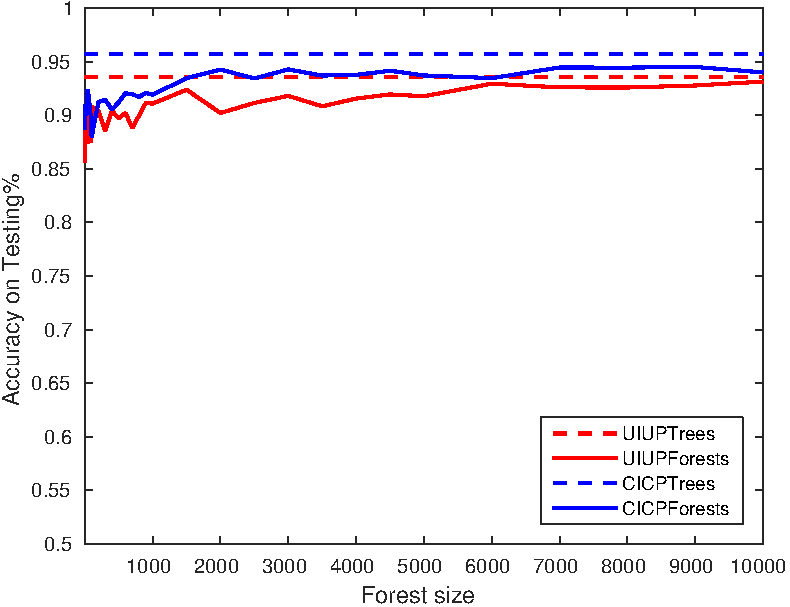
\includegraphics[width=\textwidth]{figs/PLPTF/Forests/SpectHeartDownsampledFurther_Forests_MH.pdf}
  	\caption{SpectHeart}
		\label{fig:S4}
	\end{subfigure}
  \\
  \begin{subfigure}[b]{0.3\textwidth}
		\centering
  	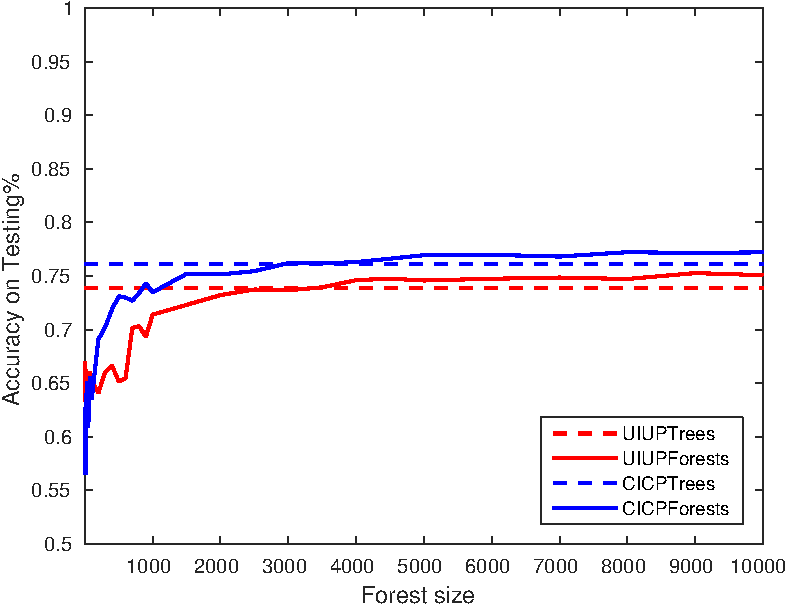
\includegraphics[width=\textwidth]{figs/PLPTF/Forests/TicTacToe_Forests_MH.pdf}
  	\caption{TicTacToe}
		\label{fig:T4}
	\end{subfigure}
  \begin{subfigure}[b]{0.3\textwidth}
		\centering
  	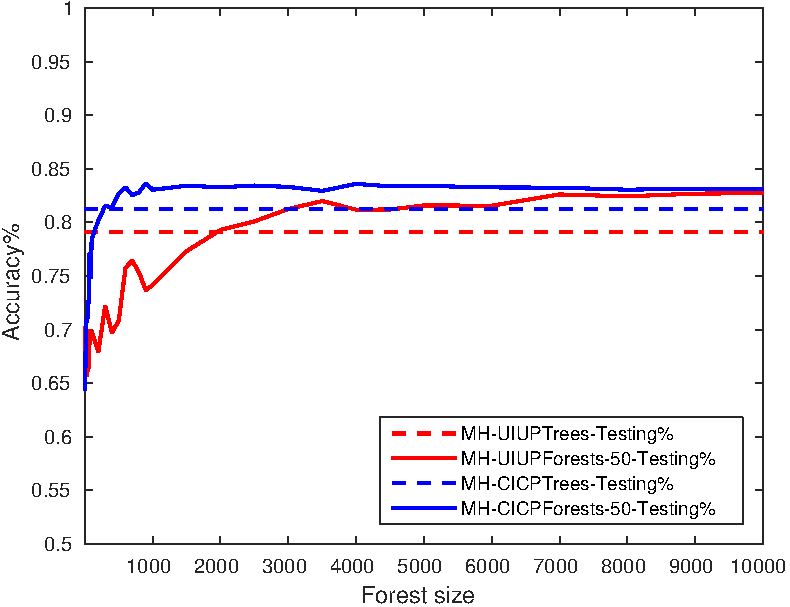
\includegraphics[width=\textwidth]{figs/PLPTF/Forests/VehicleDownsampledFurther_Forests_MH.pdf}
  	\caption{Vehicle}
		\label{fig:V4}
	\end{subfigure}
  \begin{subfigure}[b]{0.3\textwidth}
		\centering
  	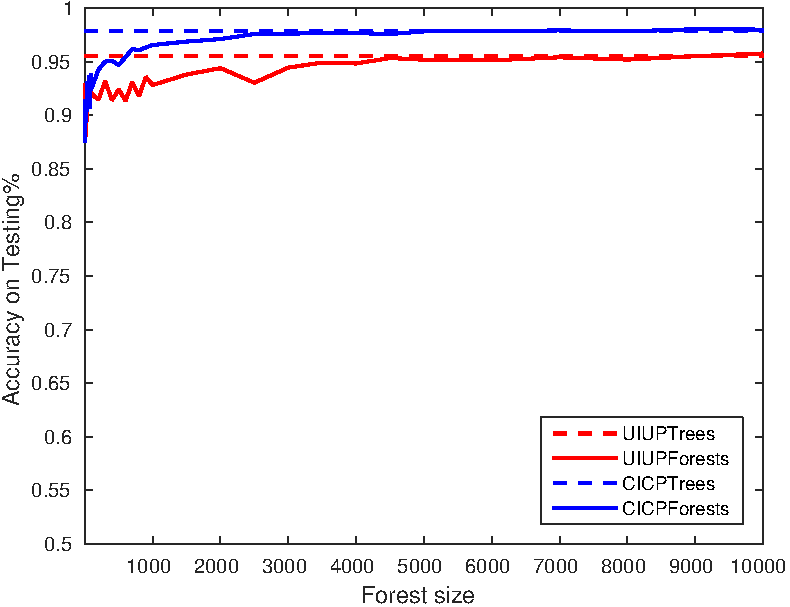
\includegraphics[width=\textwidth]{figs/PLPTF/Forests/WineDownsampled_Forests_MH.pdf}
  	\caption{Wine}
		\label{fig:W4}
	\end{subfigure}

  \caption{Learning Forests of PLP-trees with Different Sample Sizes}
  \label{fig:forests2}
\end{figure*}


\section{Conclusion}
